\ifx \notincludehead\undefined
	\newcommand*{\No}{\textnumero}
	\documentclass[russian, utf8, 12pt, pointsubsection,floatsubsection]{eskdtext}
	\usepackage[russian]{babel}

	\ifx\pdfoutput\undefined  
		\def\pdfoutput{0}
	\fi

	\ifnum\pdfoutput=0 
		\sloppy
		%	\usepackage[dvips]{graphicx}       % загрузка графики под dvi  
		\textheight=250mm                  % для DVI высота печатного текста
		\textwidth=165mm                   % ширина печатного текста
	\else
		%	\usepackage[pdftex]{graphicx}      % загрузка графики под pdf
		\usepackage{cmap}                  % чтоб работал поиск по PDF 
		% гиперссылки в PDF
		\usepackage[unicode, pdftex, colorlinks, linkcolor=blue]{hyperref} 
		\pdfcompresslevel=9                % сжимаем PDF 
		%	\textheight=240mm                  % для PDF высота печатного текста
		%	\textwidth=165mm                   % ширина печатного текста
	\fi 

	\usepackage{eskdchngsheet}
	\usepackage[T2A]{fontenc}
	%\usepackage[cp1251]{inputenc}
	\usepackage{amstext}
	\usepackage{amsmath}
	\usepackage{listings}
	\usepackage{rotating}
	\usepackage{pmasc}

	\usepackage{placeins}    % пакет позволяет вставлять плавающие объекты (рисунки) в том месте, 
                         % где это необходимо. Для вывода рисунка после него встаить команду \FloatBarrier

    \usepackage{comment}
	\usepackage{array}
	\usepackage{longtable}   % подключение длинных таблиц
    \usepackage{multirow}    % для формирования таблиц с объединением строк
	\usepackage{indentfirst} % идентификация первых абзацев после секционирования
	\usepackage{fancyhdr}                    % расширенный формат страниц
	\usepackage{ulem}        % подчеркивания текста \uline\uuline\uwave\sout \xout
	%\voffset=-25mm   % -25                   % сдвиг страницы вверх
	%\hoffset=-15mm   % -10                   % сдвиг страницы влево

	\usepackage{floatflt} % для рисунков
	\usepackage{wrapfig}  % для рисунков
    \usepackage{xcolor}
    %\usepackage[most]{tcolorbox}
    \usepackage{subcaption} % Загружает пакет заголовков
    \usepackage{xspace}

	\sloppy                             % подавление дополнительных переносов
	\righthyphenmin=2                   % можно переносить
	
	\ESKDclassCode{ТП}
	\ESKDtitle{Программная система планирования производства ПС ПП «Opti-Corrugated» \FIRMA. Подключение гофроагрегата JSM}

	\usepackage{lscape}

	% для Первой спецификации
	\ESKDdocName{Технический рабочий проект\\ Пояснительная записка.}
	\ESKDsignature{65698922.425120.00036.П2.01.1.1}
	\ESKDcolumnII{65698922.425120.00036.П2.01.1.1}
	\ESKDcolumnI{Программная документация. ТЗ. Ред.1}

	\ESKDgroup{ООО <<Опти-Софт>>}
	\ESKDauthor{Косицын Д.П.}
	\ESKDtitleAgreedBy{Директор ООО <<Опти-Софт>>}{Шабаев А.И.}
	\ESKDtitleDesignedBy{Зам. директора <<Опти-Софт>>}{Косицын Д.П.}
    \ESKDtitleDesignedBy{Консультант}{Смирнов А.В.}	
    \ESKDtitleDesignedBy{Начальник отдела разработки гофротары}{Сошкин Р.В.}


	\ESKDtitleApprovedBy{Генеральный директор \FIRMA}{\DIRECTOR}
	%\ESKDtitleApprovedBy{\rule{72pt}{1pt}}{\rule{72pt}{1pt}}
	\ESKDtitleAgreedBy{Директор по производству}{ФИО}
	%\ESKDtitleAgreedBy{Коммерческий директор}{Фамилия И.О.}
% 	\ESKDtitleAgreedBy{Финансовый директор}{Ерофеева М.А.}
% 	\ESKDtitleAgreedBy{Начальник отдела автоматизации}{ФИО}

	%\ESKDtitleAgreedBy{\rule{72pt}{1pt}}{\rule{72pt}{1pt}}

	\ESKDdate{2026/03/21}

%	\newcommand*{\No}{\textnumero}

	% для нумерации в длинных enumerate: a, b,...y, z, aa,ab,..
	%\usepackage{alphalph}  
	%\renewcommand{\theenumi}{\alphalph{\value{enumi}}}
\fi

\def \notincludehead{}

%  Текущая версия 
\newcommand{\VERSION}{1.0}


\newcommand{\FIRMA}{ООО "ДОБРЫЙ КАРТОН"}
\newcommand{\firma}{ООО "ДОБРЫЙ КАРТОН"}
\newcommand{\CURADDRESS}{450037, Республика Башкортостан, г. Уфа, Ул. Проспект Октября, дом 46}
\newcommand{\ADDRESS}{Шакша, Индустриальный парк, проезд Первый, стр. 12}
\newcommand{\ESKDNUM}{65698922.425120.063.П2.\VERSION}
\newcommand{\DIRECTOR}{Коткин Д.Е.}
\newcommand{\curobject}{}




\newcommand{\gofro}   {{@ГТ}\xspace}
\newcommand{\erp}     {{@1C:Бухгалтерия}\xspace}
% \newcommand{\buh}     {@1C:Бухгалтерия\xspace}
% \newcommand{\bhs}  {{@Syncro}\xspace}



\newcommand{\manager}     {!МенеджерПоПродажам}
\newcommand{\tehnolog}    {!Технолог}
% \newcommand{\designer}{\green{!Дизайнер}\xspace}
\newcommand{\planner}     {!Планировщик}
% % \newcommand{\montaznik}{\green{!Монтажник}\xspace}
\newcommand{\operator}    {!Оператор}
\newcommand{\linkoperator}{!ОператорРаската}
% % \newcommand{\supplier}{\green{!МенеджерПоСнабжению}\xspace}
% \newcommand{\purchase}{\green{!СпециалистПоЗакупкам}\xspace}
% \newcommand{\logistician}{\green{!МенеджерПоЛогистике}\xspace}
\newcommand{\processengineer}{!ДиректорПоПроизводству}
\newcommand{\auditor}     {!Бухгалтер}
\newcommand{\gaoperator}  {!МашинистГА}
% \newcommand{\kladovshik}{\green{!Кладовщик}\xspace}
\newcommand{\master}      {!МастерСмены}
% \newcommand{\driver}{\green{!ВодительПогрузчика}\xspace}
\newcommand{\director}    {!Директор}
\newcommand{\laborant}    {!КонтролерПоКачеству}
% \newcommand{\okk}{\green{!ОКК}\xspace}
 




%  Вариант сборки отчета 
%  1 - полная
%  0 - сокращенная
% В тексте вставить условие
%  \ifnum\curversion=1  % 1 - полная версия ТЗ
%  \input{....}
%  \fi
\newcommand{\curversion}{1} 



%\newcommand*{\No}{\textnumero}
\begin{document}
   % \include{Terms}

    % титульный лист 
   \maketitle
 	
   	\begin{center}
		\large \textbf{ИСТОРИЯ ИЗМЕНЕНИЙ} \normalsize
	\end{center}
\begin{longtable}{|p{70mm}|p{20mm}|p{20mm}|p{50mm}|}
\hline
{\bf \parbox[c][5mm]{70mm}{\centering Причина}} & {\bf \parbox[c]{20mm}{\centering Дата}} & {\bf \parbox[c]{20mm}{\centering Версия}} & {\bf \parbox[c]{50mm}{\centering Автор}} \\
\hline
\parbox[c][9mm]{70mm}{Первая редакция} & {\parbox{20mm}{20.10.2026}} & \parbox{20mm}{\curversion} & {\parbox{50mm}{}} \\
% \hline
% \parbox[c][9mm]{70mm}{Замечания по обмену с ERP} & {\parbox{20mm}{11.10.2023}} & \parbox{20mm}{1.4} & {\parbox{50mm}{Жернаков Р.В.}} \\
% \hline
% \parbox[c][9mm]{70mm}{Выслано} & {\parbox{20mm}{09.12.2023}} & \parbox{20mm}{1.1} & {\parbox{50mm}{Жернаков Р.В.}} \\
\hline
% \parbox[c][12mm]{70mm}{Внесены исправления по замечаниям. Выслано} & {\parbox{20mm}{\today}} & \parbox{20mm}{\VERTION} & {\parbox{50mm}{Жернаков Р.В.}} \\
% \hline
% \caption{}\label{}
\end{longtable}  
	
\newpage
	% содержание ЕСКД
% 		\begin{center}
		\large \textbf{СОДЕРЖАНИЕ} \normalsize
	\end{center}
	\begin{longtable}{|p{10mm}|p{10mm}|p{30mm}|p{60mm}|p{10mm}|p{25mm}|} 
	\hline

	\rotatebox{90}{\textbf{Номер строки}} &
	\rotatebox{90}{\textbf{Формат}} &
	\textbf{Обозначение} & \textbf{Наименование} & 
	\rotatebox{90}{\textbf{Кол-во листов}} & 
	\textbf{Примечание}\\
	\hline
	
	1 & A4 & & Оглавление &  & \\
	\hline
	2 & A4 & & Общие положения &  & \\
	\hline
	3 & A4 & & Назначение и цели создания системы &  & \\
	 \hline
	4 & A4 & & Характеристика объекта автоматизации &  & \\
	\hline
	5 & A4 & & Описание требований к системе &  & \\
	\hline
%	 4 & A4 & & Состав и содержание работ &  & \\
%	\hline
%	5 & A4 & & Порядок контроля и приемки работ &  & \\
%	\hline
%	 6 & A4 & & Требования к документированию &  & \\
%	\hline
%	 7 & A4 & & Приложения &  & \\
%	\hline
	\end{longtable}
%  	\newpage

	% оглавление 
	\scriptsize
	\setcounter{tocdepth}{4}
	\tableofcontents
	\normalsize
	\newpage

	% документ
    \section{Общие положения}
	\ifx \notincludehead\undefined
	\newcommand*{\No}{\textnumero}
	\documentclass[russian, utf8, 12pt, pointsubsection,floatsubsection]{eskdtext}
	\usepackage[russian]{babel}

	\ifx\pdfoutput\undefined  
		\def\pdfoutput{0}
	\fi

	\ifnum\pdfoutput=0 
		\sloppy
		%	\usepackage[dvips]{graphicx}       % загрузка графики под dvi  
		\textheight=250mm                  % для DVI высота печатного текста
		\textwidth=165mm                   % ширина печатного текста
	\else
		%	\usepackage[pdftex]{graphicx}      % загрузка графики под pdf
		\usepackage{cmap}                  % чтоб работал поиск по PDF 
		% гиперссылки в PDF
		\usepackage[unicode, pdftex, colorlinks, linkcolor=blue]{hyperref} 
		\pdfcompresslevel=9                % сжимаем PDF 
		%	\textheight=240mm                  % для PDF высота печатного текста
		%	\textwidth=165mm                   % ширина печатного текста
	\fi 

	\usepackage{eskdchngsheet}
	\usepackage[T2A]{fontenc}
	%\usepackage[cp1251]{inputenc}
	\usepackage{amstext}
	\usepackage{amsmath}
	\usepackage{listings}
	\usepackage{rotating}
	\usepackage{pmasc}

	\usepackage{placeins}    % пакет позволяет вставлять плавающие объекты (рисунки) в том месте, 
                         % где это необходимо. Для вывода рисунка после него встаить команду \FloatBarrier

    \usepackage{comment}
	\usepackage{array}
	\usepackage{longtable}   % подключение длинных таблиц
    \usepackage{multirow}    % для формирования таблиц с объединением строк
	\usepackage{indentfirst} % идентификация первых абзацев после секционирования
	\usepackage{fancyhdr}                    % расширенный формат страниц
	\usepackage{ulem}        % подчеркивания текста \uline\uuline\uwave\sout \xout
	%\voffset=-25mm   % -25                   % сдвиг страницы вверх
	%\hoffset=-15mm   % -10                   % сдвиг страницы влево

	\usepackage{floatflt} % для рисунков
	\usepackage{wrapfig}  % для рисунков
    \usepackage{xcolor}
    %\usepackage[most]{tcolorbox}
    \usepackage{subcaption} % Загружает пакет заголовков
    \usepackage{xspace}

	\sloppy                             % подавление дополнительных переносов
	\righthyphenmin=2                   % можно переносить
	
	\ESKDclassCode{ТП}
	\ESKDtitle{Программная система планирования производства ПС ПП «Opti-Corrugated» \FIRMA. Подключение гофроагрегата JSM}

	\usepackage{lscape}

	% для Первой спецификации
	\ESKDdocName{Технический рабочий проект\\ Пояснительная записка.}
	\ESKDsignature{65698922.425120.00036.П2.01.1.1}
	\ESKDcolumnII{65698922.425120.00036.П2.01.1.1}
	\ESKDcolumnI{Программная документация. ТЗ. Ред.1}

	\ESKDgroup{ООО <<Опти-Софт>>}
	\ESKDauthor{Косицын Д.П.}
	\ESKDtitleAgreedBy{Директор ООО <<Опти-Софт>>}{Шабаев А.И.}
	\ESKDtitleDesignedBy{Зам. директора <<Опти-Софт>>}{Косицын Д.П.}
    \ESKDtitleDesignedBy{Консультант}{Смирнов А.В.}	
    \ESKDtitleDesignedBy{Начальник отдела разработки гофротары}{Сошкин Р.В.}


	\ESKDtitleApprovedBy{Генеральный директор \FIRMA}{\DIRECTOR}
	%\ESKDtitleApprovedBy{\rule{72pt}{1pt}}{\rule{72pt}{1pt}}
	\ESKDtitleAgreedBy{Директор по производству}{ФИО}
	%\ESKDtitleAgreedBy{Коммерческий директор}{Фамилия И.О.}
% 	\ESKDtitleAgreedBy{Финансовый директор}{Ерофеева М.А.}
% 	\ESKDtitleAgreedBy{Начальник отдела автоматизации}{ФИО}

	%\ESKDtitleAgreedBy{\rule{72pt}{1pt}}{\rule{72pt}{1pt}}

	\ESKDdate{2026/03/21}

%	\newcommand*{\No}{\textnumero}

	% для нумерации в длинных enumerate: a, b,...y, z, aa,ab,..
	%\usepackage{alphalph}  
	%\renewcommand{\theenumi}{\alphalph{\value{enumi}}}
\fi




%\section {Общие сведения}

\begin{itemize}

    \item Полное наименование: Программная Система Планирования Производством «Opti-Corrugated» (Гофротара). Подключение гофроагрегата JSM.

    \item Краткое наименование: ПС ПП, ПС ПП «Opti-Corrugated», ПС ПП Гофротара.

    \item ЗАКАЗЧИК~--- \FIRMA.

Адрес:  \ADDRESS

    \item ИСПОЛНИТЕЛЬ: ООО <<Опти-Софт>>
Адрес: 185003, г. Петрозаводск, пр. Ленина, 31.

    \item Основание для выполнения работ: Дополнительное соглашение №3 от 03.08.2026г между \FIRMA и ООО <<Опти-Софт>>.
%\todo{Требуется уточнение}
    \item Сведения об источниках и порядке финансирования работ: финансирование за счёт средств ЗАКАЗЧИКА.

    \item Порядок сдачи работ по разработке: согласно дополнительному договору на разработку \gofro.

\end{itemize}

    \newpage

	\section{Назначение и цели создания системы}
	\ifx \notincludehead\undefined
	\newcommand*{\No}{\textnumero}
	\documentclass[russian, utf8, 12pt, pointsubsection,floatsubsection]{eskdtext}
	\usepackage[russian]{babel}

	\ifx\pdfoutput\undefined  
		\def\pdfoutput{0}
	\fi

	\ifnum\pdfoutput=0 
		\sloppy
		%	\usepackage[dvips]{graphicx}       % загрузка графики под dvi  
		\textheight=250mm                  % для DVI высота печатного текста
		\textwidth=165mm                   % ширина печатного текста
	\else
		%	\usepackage[pdftex]{graphicx}      % загрузка графики под pdf
		\usepackage{cmap}                  % чтоб работал поиск по PDF 
		% гиперссылки в PDF
		\usepackage[unicode, pdftex, colorlinks, linkcolor=blue]{hyperref} 
		\pdfcompresslevel=9                % сжимаем PDF 
		%	\textheight=240mm                  % для PDF высота печатного текста
		%	\textwidth=165mm                   % ширина печатного текста
	\fi 

	\usepackage{eskdchngsheet}
	\usepackage[T2A]{fontenc}
	%\usepackage[cp1251]{inputenc}
	\usepackage{amstext}
	\usepackage{amsmath}
	\usepackage{listings}
	\usepackage{rotating}
	\usepackage{pmasc}

	\usepackage{placeins}    % пакет позволяет вставлять плавающие объекты (рисунки) в том месте, 
                         % где это необходимо. Для вывода рисунка после него встаить команду \FloatBarrier

    \usepackage{comment}
	\usepackage{array}
	\usepackage{longtable}   % подключение длинных таблиц
    \usepackage{multirow}    % для формирования таблиц с объединением строк
	\usepackage{indentfirst} % идентификация первых абзацев после секционирования
	\usepackage{fancyhdr}                    % расширенный формат страниц
	\usepackage{ulem}        % подчеркивания текста \uline\uuline\uwave\sout \xout
	%\voffset=-25mm   % -25                   % сдвиг страницы вверх
	%\hoffset=-15mm   % -10                   % сдвиг страницы влево

	\usepackage{floatflt} % для рисунков
	\usepackage{wrapfig}  % для рисунков
    \usepackage{xcolor}
    %\usepackage[most]{tcolorbox}
    \usepackage{subcaption} % Загружает пакет заголовков
    \usepackage{xspace}

	\sloppy                             % подавление дополнительных переносов
	\righthyphenmin=2                   % можно переносить
	
	\ESKDclassCode{ТП}
	\ESKDtitle{Программная система планирования производства ПС ПП «Opti-Corrugated» \FIRMA. Подключение гофроагрегата JSM}

	\usepackage{lscape}

	% для Первой спецификации
	\ESKDdocName{Технический рабочий проект\\ Пояснительная записка.}
	\ESKDsignature{65698922.425120.00036.П2.01.1.1}
	\ESKDcolumnII{65698922.425120.00036.П2.01.1.1}
	\ESKDcolumnI{Программная документация. ТЗ. Ред.1}

	\ESKDgroup{ООО <<Опти-Софт>>}
	\ESKDauthor{Косицын Д.П.}
	\ESKDtitleAgreedBy{Директор ООО <<Опти-Софт>>}{Шабаев А.И.}
	\ESKDtitleDesignedBy{Зам. директора <<Опти-Софт>>}{Косицын Д.П.}
    \ESKDtitleDesignedBy{Консультант}{Смирнов А.В.}	
    \ESKDtitleDesignedBy{Начальник отдела разработки гофротары}{Сошкин Р.В.}


	\ESKDtitleApprovedBy{Генеральный директор \FIRMA}{\DIRECTOR}
	%\ESKDtitleApprovedBy{\rule{72pt}{1pt}}{\rule{72pt}{1pt}}
	\ESKDtitleAgreedBy{Директор по производству}{ФИО}
	%\ESKDtitleAgreedBy{Коммерческий директор}{Фамилия И.О.}
% 	\ESKDtitleAgreedBy{Финансовый директор}{Ерофеева М.А.}
% 	\ESKDtitleAgreedBy{Начальник отдела автоматизации}{ФИО}

	%\ESKDtitleAgreedBy{\rule{72pt}{1pt}}{\rule{72pt}{1pt}}

	\ESKDdate{2026/03/21}

%	\newcommand*{\No}{\textnumero}

	% для нумерации в длинных enumerate: a, b,...y, z, aa,ab,..
	%\usepackage{alphalph}  
	%\renewcommand{\theenumi}{\alphalph{\value{enumi}}}
\fi



%\section {Назначение и цели создания системы}

\subsection{Назначение системы}
Проект глубокой модернизации программной системы планирования производства ПС ПП «Opti-Corrugated» для автоматизации процессов планирования и учета производства на \FIRMA. Подключение гофроагрегата JSM-3000.




\subsection{Цели и задачи работ по разработке ПС ПП}

В рамках данного проекта модернизации программного обеспечения преследуются следующие конкретные цели применительно к документу ''Выработка гофроагрегата'':

\begin{itemize}
    \item Автоматизация запуска производства. Исключить необходимость ручного ввода времени начала смены. При открытии формы машинист должен видеть только свои задания, привязанные к оборудованию его компьютера.
        \item Интеграция с гофроагрегатом. Убрать человеческий фактор по заведению заказов в память гофроагрегата.
    \item Повышение оперативности учета. Обеспечить автоматическую регистрацию выпуска продукции и полуфабрикатов на гофроагрегате и загрузку данных в систему \gofro в режиме реального времени.

    \item Повышение точности учёта. Перейти от минут к секундам во всех расчётах длительности простоя и скорости. Скорость рассчитывать строго по чистому времени работы оборудования (исключив время пуско-наладочных работ).
    \item Обеспечение целостности данных. Добавить проверки заполнения обязательных полей перед сохранением или завершением смены. Блокировать сохранение, если не указана причина простоя или брака.
    \item Унификация интерфейсов. Реализовать единый механизм выбора причины возникновения простоя или выпуска брака с обязательным указанием пояснения. % Для быстрого добавления единичных случаев брака разработать отдельную форму.
    \item Оптимизация командной панели. На основной форме вывести кнопки для старта и завершения этапов работы (переналадка, простой), чтобы машинист мог управлять процессом вручную при необходимости.

\end{itemize}

Эти цели направлены на снижение ошибок ввода, повышение прозрачности производственного процесса и обеспечение автоматического контроля качества данных.


    \newpage

	\section{Характеристика объекта автоматизации}
	\ifx \notincludehead\undefined
	\newcommand*{\No}{\textnumero}
	\documentclass[russian, utf8, 12pt, pointsubsection,floatsubsection]{eskdtext}
	\usepackage[russian]{babel}

	\ifx\pdfoutput\undefined  
		\def\pdfoutput{0}
	\fi

	\ifnum\pdfoutput=0 
		\sloppy
		%	\usepackage[dvips]{graphicx}       % загрузка графики под dvi  
		\textheight=250mm                  % для DVI высота печатного текста
		\textwidth=165mm                   % ширина печатного текста
	\else
		%	\usepackage[pdftex]{graphicx}      % загрузка графики под pdf
		\usepackage{cmap}                  % чтоб работал поиск по PDF 
		% гиперссылки в PDF
		\usepackage[unicode, pdftex, colorlinks, linkcolor=blue]{hyperref} 
		\pdfcompresslevel=9                % сжимаем PDF 
		%	\textheight=240mm                  % для PDF высота печатного текста
		%	\textwidth=165mm                   % ширина печатного текста
	\fi 

	\usepackage{eskdchngsheet}
	\usepackage[T2A]{fontenc}
	%\usepackage[cp1251]{inputenc}
	\usepackage{amstext}
	\usepackage{amsmath}
	\usepackage{listings}
	\usepackage{rotating}
	\usepackage{pmasc}

	\usepackage{placeins}    % пакет позволяет вставлять плавающие объекты (рисунки) в том месте, 
                         % где это необходимо. Для вывода рисунка после него встаить команду \FloatBarrier

    \usepackage{comment}
	\usepackage{array}
	\usepackage{longtable}   % подключение длинных таблиц
    \usepackage{multirow}    % для формирования таблиц с объединением строк
	\usepackage{indentfirst} % идентификация первых абзацев после секционирования
	\usepackage{fancyhdr}                    % расширенный формат страниц
	\usepackage{ulem}        % подчеркивания текста \uline\uuline\uwave\sout \xout
	%\voffset=-25mm   % -25                   % сдвиг страницы вверх
	%\hoffset=-15mm   % -10                   % сдвиг страницы влево

	\usepackage{floatflt} % для рисунков
	\usepackage{wrapfig}  % для рисунков
    \usepackage{xcolor}
    %\usepackage[most]{tcolorbox}
    \usepackage{subcaption} % Загружает пакет заголовков
    \usepackage{xspace}

	\sloppy                             % подавление дополнительных переносов
	\righthyphenmin=2                   % можно переносить
	
	\ESKDclassCode{ТП}
	\ESKDtitle{Программная система планирования производства ПС ПП «Opti-Corrugated» \FIRMA. Подключение гофроагрегата JSM}

	\usepackage{lscape}

	% для Первой спецификации
	\ESKDdocName{Технический рабочий проект\\ Пояснительная записка.}
	\ESKDsignature{65698922.425120.00036.П2.01.1.1}
	\ESKDcolumnII{65698922.425120.00036.П2.01.1.1}
	\ESKDcolumnI{Программная документация. ТЗ. Ред.1}

	\ESKDgroup{ООО <<Опти-Софт>>}
	\ESKDauthor{Косицын Д.П.}
	\ESKDtitleAgreedBy{Директор ООО <<Опти-Софт>>}{Шабаев А.И.}
	\ESKDtitleDesignedBy{Зам. директора <<Опти-Софт>>}{Косицын Д.П.}
    \ESKDtitleDesignedBy{Консультант}{Смирнов А.В.}	
    \ESKDtitleDesignedBy{Начальник отдела разработки гофротары}{Сошкин Р.В.}


	\ESKDtitleApprovedBy{Генеральный директор \FIRMA}{\DIRECTOR}
	%\ESKDtitleApprovedBy{\rule{72pt}{1pt}}{\rule{72pt}{1pt}}
	\ESKDtitleAgreedBy{Директор по производству}{ФИО}
	%\ESKDtitleAgreedBy{Коммерческий директор}{Фамилия И.О.}
% 	\ESKDtitleAgreedBy{Финансовый директор}{Ерофеева М.А.}
% 	\ESKDtitleAgreedBy{Начальник отдела автоматизации}{ФИО}

	%\ESKDtitleAgreedBy{\rule{72pt}{1pt}}{\rule{72pt}{1pt}}

	\ESKDdate{2026/03/21}

%	\newcommand*{\No}{\textnumero}

	% для нумерации в длинных enumerate: a, b,...y, z, aa,ab,..
	%\usepackage{alphalph}  
	%\renewcommand{\theenumi}{\alphalph{\value{enumi}}}
\fi



%\section {Характеристика объектов автоматизации}
\FIRMA (ПРЕДПРИЯТИЕ)~--- это предприятие, выпускающее транспортную гофроупаковку для различных отраслей промышленности. Предприятие предлагает широкий ассортимент продукции высокого качества~--- упаковку любой конструкции из трехслойного гофрокартона профиля B и С, и пятислойного картона ВС. Основной целью деятельности ПРЕДПРИЯТИЯ является получение прибыли за счет изготовления товарного гофрокартона и ящиков по заказам коммерческих предприятий.

    \newpage

% Общие требования
    %\input{main_requirement}

	% перечень модулей системы и их характеристики
    \newpage
%\section{Описание требований к системе}
%
%В системе требуется добавить реализацию следующих модулей.

	% \input{10_Modules/Mod_sales.tex}
	\subsection{Требования по модулю ''Учет технологических карт''}
\label{sec:design}

% Справочник  
\subsection{Справочник <<Оборудование>>}
\label{spr:eqpt}


\subsubsection{Описание предметной области}

Справочник <<Оборудование>> содержит информацию о технологическом оборудовании на предприятии.

Справочник уже существует в СИСТЕМЕ, требуется внести изменения в его работу.

\subsubsection{Атрибуты}

В справочнике должны быть добавлены следующие поля.

\pc
\begin{longtable}{|p{50mm}|p{30mm}|p{78mm}|}
\hline
{\bf Наименование} & {\bf Тип данных} &  {\bf Комментарий} \endhead
\hline 
   Обмен с гофроагрегатом & Булево & Признак использования Обмена с гофроагрегатом \\
   \hline
   ТипРилевокПоУмолчанию & Перечисление. ТипыРилевок & Тип Рилевок По Умолчанию \\
   \hline
   ИнтервалОпросаБД & Число (10) & Интервал опроса БД, сек \\
   \hline
   СтрокаСоединенияСБД & Строка(0) & Строка соединения с БД системы ACS \\
   \hline
\caption{Описание свойств объекта <<Оборудование>>.}
\label{tab:tdb_eqpt}
\end{longtable} 


% \item Установлен флаг «Обмен с гофроагрегатом» – влияет на доступность команд обмена в документе выработки;
% \item ID Пустого контрагента – идентификатор контрагента, который будет подставляться для пустого заказа в раскрое (см. «Общие правила формирования заданий», п.3.2);
% \item Интервал опроса БД, сек. – частота обновления данных из базы JSDCS;



\subsubsection{Функциональные требования}

\point{Изменить форму ''Оборудование''} 

Добавить вкладку Обмен ACS. 
На вкладке расположить новые поля таблицы \ref{tab:tdb_eqpt}.

Строка подключения с БД – параметры подключения к базе asc\_dev, где:
 \begin{itemize}
     \item DRIVER –-- тип СУБД (MS SQL, MySQL и т.д.);
     \item SERVER --– адрес базы данных ACS в сети предприятия;
     \item ID –-- имя пользователя (По умолчанию  для asc\_dev ''sa'');
     \item PWD –-- пароль (По умолчанию  для asc\_dev ''sa'');
     \item DATABASE –-- имя базы данных (По умолчанию для asc\_dev ''asc\_dev'');
\end{itemize}

Добавить на вкладке Обмен ACS новую вкладку ''Проверка работы с JSM''



\point{Проверить соединение с JSM}

Добавить команду ''Проверить соединение с JSM''.
По команде пользователя необходимо выполнить тестовое подключение к базе данных JSM.

В случае неуспешного подключения необходимо выдавать сообщение об ошибке подключения.



\point{Получить данные с JSM}

По команде ''Получить данные с JSM'' система должна получить из памяти JSM текущие данные по выработки 
гофроагрегата. 

Результаты запроса должны быть выведены в отдельное поле на форме ''Результат запроса''.

\subsection{Справочник <<Слои картона>>}
\label{spr:Layer}

\subsubsection{Описание предметной области}

Справочник существует в СИСТЕМЕ, необходимо внести изменения в функциональность.

\subsubsection{Атрибуты}

В справочнике должны быть добавлены следующие поля.

\pc
\begin{longtable}{|p{50mm}|p{30mm}|p{78mm}|}
\hline
{\bf Наименование} & {\bf Тип данных} &  {\bf Комментарий} \endhead
\hline 
   КодACS & Строка(2) & Код картона в системе ACS гофроагрегата JSM. Код всегда должен состоять из двух символов: первый – литера, второй – цифра. \\
   \hline
\caption{Описание свойств объекта <<Оборудование>>.}
\label{tab:tdb_eqpt}
\end{longtable} 


% Перечисления

\subsection{Перечисление <<ТипыРилевок>>}
\label{spr:ScoreType}

Значение Типа рилёвок:
\begin{itemize}
    \item 1 = ПапаМама
    \item 2 = ПапаПлоский
    \item 3 = ПапаПапа
\end{itemize}

%	\input{10_Modules/Modules2.tex}
%	\input{10_Modules/Mod_Planing.tex}
	% Документ  
\subsection{Документ <<Выработка гофроагрегата>>}
\label{doc:Doc_ProdGA}

% \subsubsection{Атрибуты}


% В документ необходимо добавить следующие колонки табличной части <<Раскрои>>.

% \pc
% \begin{longtable}{|p{4cm}|p{4cm}|p{8cm}|}
% \hline
% {\bf Наименование} & {\bf Тип данных} &  {\bf Комментарий} \endhead
%     \hline
%     Менеджер & Справочник <<Физические лица>> & Менеджер, который создал заказ на выпуск данного изделия. Подтягивается из заявки текущего заказа. Закрыто для редактирования.\\
%     \hline
%     Номер связки & Число (10,0) & Номер связки раскроя для выгрузки в память гофроагрегата.\\
%     \hline   
%    \caption{Новые колонки табличной части <<Раскрои>>}
%   \label{tab:ProdGA}
% \end{longtable}

\subsubsection{Функциональные требования}

\point{Изменить форму документа}

Добавить группу команд по связи с гофроагрегатом.
Добавить в группу индикатор состояния подключения к гофроагрегату.
При положительном подключении индикатор после выполнения команды НачатьЧтениеДанныхГА должен показывать статус подключения к ГА.
При отрицательном подключении индикатор должен показывать красный сигнал ошибки.

Форма редактирования документа представлена на рисунке \ref{fig:placeholder}.
\begin{figure}[h]
    \centering
    \fbox{
    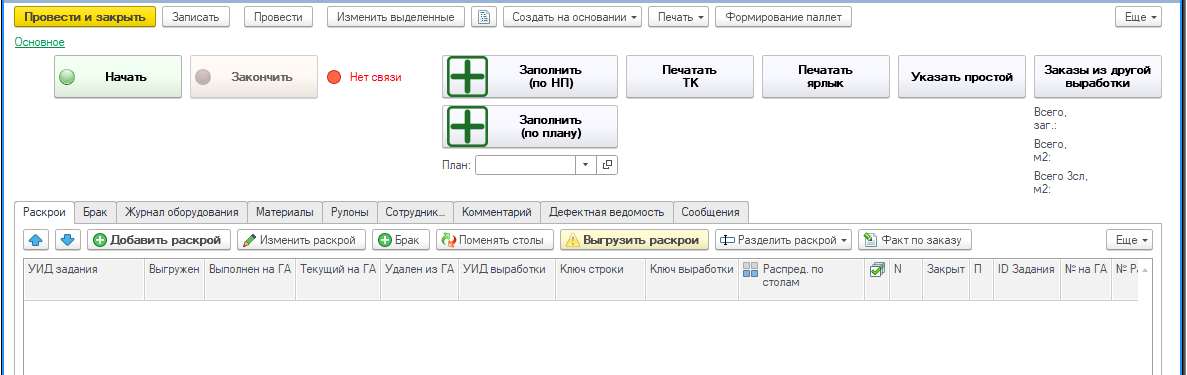
\includegraphics[height=0.21 \textheight, keepaspectratio]{50_Pics/Doc_ProdGA.png}}
    \caption{Измененная форма редактирования документа}
    \label{fig:placeholder}
\end{figure}


\point{Добавить команду ''Выгрузить раскрои''}

В документе <<Выработка гофроагрегата>> в табличной части <<Раскрои>> добавить команду ''Выгрузить раскрои''.
Выделенные пользователем в табличной части ''Раскрои'' должны быть по команде выгружены в память гофроагрегата JSM.
Для выгруженного задания должен быть указан признак ''Выгружен'' Истина.
При повторной выгрузке задание не должно быть выгружено без удаления на стороне JSM.


\point{Добавить команду ''Начать чтение данных ГА''}

По команде система должна начать считывать данные с ГА согласно функции \ref{sec:startreading} ''Начать чтение данных с ГА''. Статус подключения должен измениться на ''Подключен''.


\point{Добавить команду ''Закончить чтение данных ГА''}

По команде система должна закончить считывать данные с ГА согласно функции \ref{sec:stopreading} ''Закончить чтение данных с ГА''. Статус подключения должен измениться на ''Нет связи''.



%	\input{10_Modules/Mod_Shipment.tex}
%	
	\subsection{Требования по организации обмена данными с системами управления гофроагрегатом J.S.Machine}
\label{sec:BHS}

СИСТЕМА должна обмениваться данными с системами управления гофроагрегатом J.S.Machine. Программа управления заказами - ACS.

Обмен данными должен производиться из формы редактирования документа ''Выработка гофроагрегата'' (см. \ref{doc:Doc_ProdGA}).

\subsubsection{Настройка подключения для оборудования}

Для подключения к гофроагрегату J.S.Machine (Программа управления заказами - ACS)
в параметрах справочника ''Оборудование'' для гофроагрегата J.S.M. должны быть заполненные следующие данные.

\begin{enumerate}
\item Установлен флаг «Обмен с гофроагрегатом» – влияет на доступность команд обмена в документе выработки;
\item Интервал опроса БД, сек. – частота обновления данных из базы ACS;
\item Строка подключения с БД – параметры подключения к базе ACS, где:
\begin{itemize}
    \item DRIVER –- тип СУБД (MS SQL, MySQL и т.д.);
    \item SERVER –- адрес базы данных ACS в сети предприятия;
    \item ID –- имя пользователя (По умолчанию  для ACS ''sa'');
    \item PWD –- пароль (По умолчанию  для ACS ''sa'');
    \item DATABASE –- имя базы данных (По умолчанию для ACS ''[asc\_dev]'');
     
\end{itemize}
\end{enumerate}


\subsubsection{Структура файлов на JSACS}

% \setCJKmainfont{SimSun}
% \begin{CJK*}{UTF8}{zhsong}
Основные таблицы для работы

\point{Таблица Acs\_Order}

Таблица, содержащая список раскроев и их параметров.

% \begin{itemize}
%     \item fID – идентификатор раскроя (ID Задания);
%  \item 	Web – формат;
%  \item 	Remark – комментарий;
%  \item 	Trim – кромка;
%  \item 	Linedepth – глубина рилёвки;
%  \item 	SN – порядковый номер раскроя;
%  \item 	user\_fID – идентификатор пользователя;
%  \item 	AuditFields\_InsertDate – дата создания;
%  \item 	AuditFields\_UpdateDate – дата изменения;
%  \item 	LineType\_fID – идентификатор типа рилёвки (всегда равен 1);
%  \item 	Finished – признак, что раскрой был выполнен;
%  \item 	ChangSpd, BestSpd, maxSpd – параметры скорости работы;
%  \item 	Cust\_SN – порядковый номер (задаётся аналогично полю SN);
%  \item 	Cust\_SchNo – номер плана (не указывается);
%  \item 	Cust\_ProdNo – артикул (не указывается);
%  \item 	PaperMass\_fID – композиция;
%  \item 	PaperMassFlute\_fID – идентификатор профиля.
% \end{itemize}


% Table generated by Excel2LaTeX from sheet 'Раскрои'
\scriptsize
\begin{longtable}{|p{56mm}|p{56mm}|p{56mm}|}
\hline
{\bf \parbox[c][5mm]{56mm}{\centeringПоле}} & {\bf \parbox[c]{56mm}{\centeringТип}} & {\bf \parbox[c]{56mm}{\centeringПримечание}} \\
\hline
\parbox[c][5mm]{56mm}{Id} & \parbox{56mm}{Уникальный идентификатор} & \parbox{56mm}{Идентификатор Раскроя} \\
\hline
\parbox[c][5mm]{56mm}{Sn} & \parbox{56mm}{Число (4, 0)} & \parbox{56mm}{Порядковый номер Раскроя (10 - 9999)} \\
\hline
\parbox[c][5mm]{56mm}{OrderId} & \parbox{56mm}{Число (10, 0)} & \parbox{56mm}{Номер Раскроя} \\
\hline
\parbox[c][5mm]{56mm}{Web} & \parbox{56mm}{Число (4, 0)} & \parbox{56mm}{Формат} \\
\hline
\parbox[c][5mm]{56mm}{Trim} & \parbox{56mm}{Число (10, 4)} & \parbox{56mm}{Обрезь, мм} \\
\hline
\parbox[c][5mm]{56mm}{Trimmed} & \parbox{56mm}{Число (1, 0)} & \parbox{56mm}{Признак ''Без обрези''} \\
\hline
\parbox[c][5mm]{56mm}{Linedepth} & \parbox{56mm}{Число (10, 4)} & \parbox{56mm}{Глубина рилёвки, мм * 10} \\
\hline
\parbox[c][5mm]{56mm}{PaperMassGuid} & \parbox{56mm}{Уникальный идентификатор} & \parbox{56mm}{Идентификатор Композиции} \\
\hline
\parbox[c][5mm]{56mm}{PaperMassCode} & \parbox{56mm}{Строка (50)} & \parbox{56mm}{Наименование Композиции} \\
\hline
\parbox[c][5mm]{56mm}{PaperMassFluteGuid} & \parbox{56mm}{Уникальный идентификатор} & \parbox{56mm}{Идентификатор Профиля} \\
\hline
\parbox[c][5mm]{56mm}{FluteCode} & \parbox{56mm}{Строка (50)} & \parbox{56mm}{Наименование Профиля} \\
\hline
\parbox[c][5mm]{56mm}{LineTypeGuid} & \parbox{56mm}{Уникальный идентификатор} & \parbox{56mm}{Идентификатор Типа рилёвок} \\
\hline
\parbox[c][21mm]{56mm}{LineTypeValue} & \parbox{56mm}{Число (1, 0)} & \parbox{56mm}{Значение Типа рилёвок: 1 = ПапаМама; 2 = ПапаПлоский; 3 = ПапаПапа} \\
\hline
\parbox[c][5mm]{56mm}{LineTypeCode} & \parbox{56mm}{Строка (50)} & \parbox{56mm}{Наименование Типа рилёвок} \\
\hline
\parbox[c][5mm]{56mm}{Finished} & \parbox{56mm}{Число (1, 0)} & \parbox{56mm}{Признак завершённого Раскроя} \\
\hline
\parbox[c][5mm]{56mm}{ChangSpd} & \parbox{56mm}{Число (4, 0)} & \parbox{56mm}{Значение = 200} \\
\hline
\parbox[c][5mm]{56mm}{BestSpd} & \parbox{56mm}{Число (4, 0)} & \parbox{56mm}{Значение = 240} \\
\hline
\parbox[c][5mm]{56mm}{MaxSpd} & \parbox{56mm}{Число (4, 0)} & \parbox{56mm}{Значение = 200} \\
\hline
\parbox[c][5mm]{56mm}{PrePress} & \parbox{56mm}{Число (1, 0)} & \parbox{56mm}{Значение = 0} \\
\hline
\caption{Таблица Acs\_Order}\label{tab:Acs_Order}
\end{longtable}  
\normalsize


\point{Таблица 	Acs\_OrderItem}

Таблица, содержащая список заказов в раскроях.

% Table generated by Excel2LaTeX from sheet 'Заказы'
\scriptsize
\begin{longtable}{|p{56mm}|p{56mm}|p{56mm}|}
\hline
{\bf \parbox[c][5mm]{56mm}{\centeringПоле}} & {\bf \parbox[c]{56mm}{\centeringТип}} & {\bf \parbox[c]{56mm}{\centeringПримечание}} \\
\hline
\parbox[c][5mm]{56mm}{Id} & \parbox{56mm}{Уникальный идентификатор} & \parbox{56mm}{Идентификатор Заказа} \\
\hline
\parbox[c][5mm]{56mm}{OrderId} & \parbox{56mm}{Число (10, 0)} & \parbox{56mm}{Номер Раскроя} \\
\hline
\parbox[c][5mm]{56mm}{OrderItemId} & \parbox{56mm}{Число (10, 0)} & \parbox{56mm}{Номер Заказа} \\
\hline
\parbox[c][5mm]{56mm}{OrderGuid} & \parbox{56mm}{Уникальный идентификатор} & \parbox{56mm}{Идентификатор Раскроя} \\
\hline
\parbox[c][5mm]{56mm}{CustomerGuid} & \parbox{56mm}{Уникальный идентификатор} & \parbox{56mm}{Идентификатор Контрагента} \\
\hline
\parbox[c][5mm]{56mm}{CustomerID} & \parbox{56mm}{Строка (100)} & \parbox{56mm}{Код Контрагента} \\
\hline
\parbox[c][5mm]{56mm}{CustomerCode} & \parbox{56mm}{Строка (100)} & \parbox{56mm}{Наименование Контрагента} \\
\hline
\parbox[c][5mm]{56mm}{Sec} & \parbox{56mm}{Число (1, 0)} & \parbox{56mm}{Количество полос} \\
\hline
\parbox[c][5mm]{56mm}{StkModelGuid} & \parbox{56mm}{Уникальный идентификатор} & \parbox{56mm}{Идентификатор упаковки} \\
\hline
\parbox[c][5mm]{56mm}{StkModelCode} & \parbox{56mm}{Строка (100)} & \parbox{56mm}{Наименование упаковки} \\
\hline
\parbox[c][5mm]{56mm}{Length} & \parbox{56mm}{Число (10, 0)} & \parbox{56mm}{Длина заготовки, мм} \\
\hline
\parbox[c][5mm]{56mm}{Width} & \parbox{56mm}{Число (10, 4)} & \parbox{56mm}{Ширина заготовки, мм} \\
\hline
\parbox[c][5mm]{56mm}{Stk} & \parbox{56mm}{Число (10, 0)} & \parbox{56mm}{Количество в пачке} \\
\hline
\parbox[c][5mm]{56mm}{Qty} & \parbox{56mm}{Число (10, 0)} & \parbox{56mm}{Количество резов} \\
\hline
\parbox[c][10mm]{56mm}{StkNumber} & \parbox{56mm}{Число (4, 0)} & \parbox{56mm}{Количество пачек (по умолчанию = 20)} \\
\hline
\parbox[c][15mm]{56mm}{Level} & \parbox{56mm}{Число (1, 0)} & \parbox{56mm}{Стол: 0 = Верхний 1 = Нижний} \\
\hline
\parbox[c][5mm]{56mm}{IsNorMal} & \parbox{56mm}{Число (1, 0)} & \parbox{56mm}{Значение = 1} \\
\hline
\parbox[c][5mm]{56mm}{Lines} & \parbox{56mm}{Строка (100)} & \parbox{56mm}{Строка рилёвок} \\
\hline
\parbox[c][5mm]{56mm}{CustOrderId} & \parbox{56mm}{Число (1, 0)} & \parbox{56mm}{Значение = 1} \\
\hline
\parbox[c][5mm]{56mm}{ProductName} & \parbox{56mm}{Строка (100)} & \parbox{56mm}{Наименование изделия} \\
\hline
\parbox[c][5mm]{56mm}{PlanSheet} & \parbox{56mm}{Строка (100)} & \parbox{56mm}{Номер Плана} \\
\hline
\parbox[c][5mm]{56mm}{PlanFinishedDate} & \parbox{56mm}{Дата} & \parbox{56mm}{Плановая дата завершения} \\
\hline
\parbox[c][5mm]{56mm}{IsPaperBox} & \parbox{56mm}{Число (1, 0)} & \parbox{56mm}{Значение = 0} \\
\hline
\parbox[c][5mm]{56mm}{IsQuickOut} & \parbox{56mm}{Число (1, 0)} & \parbox{56mm}{Значение = 0} \\
\hline
\parbox[c][5mm]{56mm}{Sn} & \parbox{56mm}{Число (4, 0)} & \parbox{56mm}{Порядковый номер Раскроя} \\
\hline
\parbox[c][5mm]{56mm}{OutPaperPath} & \parbox{56mm}{Число (1, 0)} & \parbox{56mm}{Значение = 0} \\
\hline
\parbox[c][5mm]{56mm}{Trim} & \parbox{56mm}{Число (10, 4)} & \parbox{56mm}{Обрезь, мм} \\
\hline
\parbox[c][5mm]{56mm}{Web} & \parbox{56mm}{Число (4, 0)} & \parbox{56mm}{Формат} \\
\hline
\parbox[c][5mm]{56mm}{StkModelValue} & \parbox{56mm}{Число (1, 0)} & \parbox{56mm}{Значение = 0} \\
\hline
\parbox[c][5mm]{56mm}{OrderStaus} & \parbox{56mm}{Число (1, 0)} & \parbox{56mm}{Значение = 0?} \\
\hline
\caption{Таблица Acs\_OrderItem}\label{tab:Acs_OrderItem}
\end{longtable}  
\normalsize




\point{Таблица 	Acs\_CompleteOrder	}

Таблица, содержащая информацию о выполненных раскроях.

% Table generated by Excel2LaTeX from sheet 'Данные выработки'
\scriptsize
\begin{longtable}{|p{56mm}|p{56mm}|p{56mm}|}
\hline
{\bf \parbox[c][5mm]{56mm}{\centeringПоле}} & {\bf \parbox[c]{56mm}{\centeringТип}} & {\bf \parbox[c]{56mm}{\centeringПримечание}} \\
\hline
\parbox[c][5mm]{56mm}{Sn} & \parbox{56mm}{Число (4, 0)} & \parbox{56mm}{Номер раскроя на ГА} \\
\hline
\parbox[c][5mm]{56mm}{OrderGuid} & \parbox{56mm}{Уникальный идентификатор} & \parbox{56mm}{УИД строки Раскроя} \\
\hline
\parbox[c][5mm]{56mm}{OrderItemGuid} & \parbox{56mm}{Уникальный идентификатор} & \parbox{56mm}{УИД строки Заказа} \\
\hline
\parbox[c][5mm]{56mm}{StartTime} & \parbox{56mm}{Дата} & \parbox{56mm}{Дата начала выработки} \\
\hline
\parbox[c][5mm]{56mm}{EndTime} & \parbox{56mm}{Дата} & \parbox{56mm}{Дата окончания выработки} \\
\hline
\parbox[c][10mm]{56mm}{ProdQty} & \parbox{56mm}{Число (10, 0)} & \parbox{56mm}{Количество выпущенных заготовок, шт.} \\
\hline
\parbox[c][10mm]{56mm}{WastQty} & \parbox{56mm}{Число (10, 0)} & \parbox{56mm}{Количество бракованных заготовок, шт.} \\
\hline
\parbox[c][26mm]{56mm}{StopTime} & \parbox{56mm}{Число (10, 0)} & \parbox{56mm}{Общее время простоя, сек.
(Если значение <> 0, то в Журнал работы оборудования будет добавлена запись о простое)} \\
\hline
\caption{Таблица Acs\_CompleteOrder} \label{tab:Acs_CompleteOrder}
\end{longtable}  
\normalsize

 
 
%В данной таблице всегда отображается половина выполняемого раскроя в текущий момент. Например, если раскрой состоит из двух заказов, здесь будет строчка второго заказа с оперативно обновляемым фактом выработки, в то время как строки первого заказа нет. Однако, как только раскрой завершится, факт выработки по обоим заказам отразится корректно. Вероятно, эта особенность является недоработкой со стороны ACS.

\point{Таблица 	Acs\_ProdPresses	} 

Таблица, содержащая информацию о текущих данных выработки.

% ВНИМАНИЕ. Гофроагрегат J.S.Machine и система DCS записывает данные в указанную таблицу по раскроям ТОЛЬКО ПО ФАКТУ ОКОНЧАНИЯ ВЫПОЛНЕНИЯ РАСКРОЯ. 
% Промежуточная информация по раскрою НЕДОСТУПНА.

% Table generated by Excel2LaTeX from sheet 'Текущие данные'
\scriptsize
\begin{longtable}{|p{56mm}|p{56mm}|p{56mm}|}
\hline
{\bf \parbox[c][5mm]{56mm}{\centeringПоле}} & {\bf \parbox[c]{56mm}{\centeringТип}} & {\bf \parbox[c]{56mm}{\centeringПримечание}} \\
\hline
\parbox[c][5mm]{56mm}{OrderItemGuid} & \parbox{56mm}{Уникальный идентификатор} & \parbox{56mm}{УИД строки Заказа} \\
\hline
\parbox[c][5mm]{56mm}{StartTime} & \parbox{56mm}{Дата} & \parbox{56mm}{Дата начала выработки} \\
\hline
\parbox[c][5mm]{56mm}{EndTime} & \parbox{56mm}{Дата} & \parbox{56mm}{Дата окончания выработки} \\
\hline
\parbox[c][10mm]{56mm}{ProdArea} & \parbox{56mm}{Число (18, 4)} & \parbox{56mm}{Площадь выпущенных заготовок, м2} \\
\hline
\parbox[c][10mm]{56mm}{BadArea} & \parbox{56mm}{Число (18, 4)} & \parbox{56mm}{Площадь бракованных заготовок, м2} \\
\hline
\caption{Таблица Acs\_ProdPresses}\label{tab:Acs_ProdPresses}
\end{longtable}  
\normalsize




Данная таблица всегда содержит N+1 строк, где N – количество заказов в раскрое. Последняя строка отражает суммарные данные по смене.


% \end{CJK*}

% Для выгрузки в память гофроагрегата СИСТЕМА выгружает файл с производственными заказами и раскроями в общую папку компьютера гофроагрегата. 
% Имя общей папки --- ''IPAddress/RcvOrder'' или ''ComputerName/RcvOrder'',
% где IPAddress  -- IP-адрес компьютера с утсновленонй системой DCS, ComputerName -- сетевое имя компьютера DCS.
% Папка RcvOrder должна находится в корневом каталоге диска D компьютера DCS.

%  СИСТЕМА должна иметь доступ к общей папке. Кодировка файлов --- ASCII. Каждая строка в файлах должна заканчиваться стандартной комбинацией символов конца строки (0x0D, 0x0A). Строка состоит из последовательности полей. Отдельное поле представляет собой комбинацию символов. Используемые форматы полей представлены в таблице \ref{tab:jlm_structure_of_output}.

% DCS считывает и удаляет текст OfficeH.txt

%\scriptsize
%\pc
%\begin{longtable}{|p{20mm}|p{40mm}|p{60mm}|}
%\hline
%{\bf Обозначение} & {\bf Тип значения} & {\bf } \endhead
%\hline AN & буквенно-цифровой & значение выравнено по левому краю\\
%\hline N & числовой & значение выравнено по правому краю\\
%\hline N/B & числовой или пустой & значение выравнено по правому краю\\
%\hline D & дата (ГГГГММДД) & значение состоит из 8 цифр\\
%\hline T & время (ЧЧММСС) & значение состоит из 6 цифр\\
%\hline ID & идентификатор установки & значение состоит из 20 знаков\\
%\hline PID & идентификатор бумаги & значение состоит из 44 знаков\\
%\hline
%\caption{Форматы полей, используемые в файлах обмена с гофроагрегатами BHS}
%\label{tab:bhs_formats_of_fields}
%\end{longtable} 
%
%\normalsize
%
%Идентификатор установки всегда состоит из 20 знаков. Структура идентификатора установки представлена в таблице \ref{tab:bhs_structure_of_id}.
%
%\scriptsize
%\pc
%\begin{longtable}{|p{20mm}|p{80mm}|p{20mm}|}
%\hline
%{\bf Длина} & {\bf Значение} & {\bf Формат} \endhead
%\hline 16 & идентификатор установки & AN\\
%\hline 3 & серийный номер & N/B\\
%\hline 1 & идентификатор этапа работы гофроагрегата по заданной установке & N/B\\
%\hline
%\caption{Структура идентификатора установки}
%\label{tab:bhs_structure_of_id}
%\end{longtable}
%
%\normalsize
%
%Идентификатор этапа работы гофроагрегата по заданной установке используется в ситуациях, когда работа гофроагрегата по заданной установке разделяется на этапы. Например, работа гофроагрегата по заданной установке останавливается вечером и возобновляется утром. В такой ситуации идентификатор уже выполненного этапа работы гофроагрегата может быть равен 1, а идентификатор еще невыполненного этапа –-- 2.
%
%Идентификатор бумаги всегда состоит из 44 знаков. Структура идентификатора бумаги представлена в таблице \ref{tab:bhs_structure_of_pid}.
%
%\scriptsize
%\pc
%\begin{longtable}{|p{20mm}|p{80mm}|p{20mm}|}
%\hline
%{\bf Длина} & {\bf Значение} & {\bf Формат} \endhead
%\hline 20 & код бумаги & AN\\
%\hline 4 & плотность бумаги (г/м$^2$) & N\\
%\hline 20 & наименование бумаги (дополнительные коды) & AN/B\\
%\hline
%\caption{Структура идентификатора бумаги}
%\label{tab:bhs_structure_of_pid}
%\end{longtable}
%
%\normalsize



\subsubsection{Функциональные требования}

\point{Выгрузить раскрои в J.S.Machine}

Выгружать СИСТЕМА должна раскрои без признака ''Выгружен''. В форме редактирования документа ''Выработка гофроагрегата'' в табличной части ''Раскрои'' СИСТЕМА должна позволять выделять строки (несколько строк) раскроев. 
По нажатию на кнопку ''Выгрузить раскрои'' СИСТЕМА должна 
автоматически подключаться к базе данных гофроагрега и выгрузить отмеченные раскрои. У выгруженных раскроев заполнится поле «Номер связки» – это порядковый номер раскроя в очереди гофроагрегата. 


Выгруженные раскрои должны быть помечены в таблице  признаком ''Выгружен''. 

В течение смены новые раскрои могут также добавляться и выгружаться без необходимости остановки чтения данных гофроагрегата.


Для формирования запроса требуется следующая структура данных:
\pc
\begin{longtable}{|p{4cm}|p{4cm}|p{8cm}|}
\hline
{\bf Наименование} & {\bf Тип данных} &  {\bf Комментарий} \endhead
    \hline
    УИД раскроя &	Уникальный идентификатор	& Уникальный идентификатор Раскроя \\
    \hline
    Номер раскроя &	Строка (50)	& ID Задания \\
    \hline
    Композиция &	Строка (50)&	Композиция раскроя, состоящая из кодов слоёв
(см.  "Общие правила формирования заданий", п.4)\\
    \hline
    Профиль &	Строка (50)&	 \\
    \hline
    Формат &	Число (4, 0)	 \\
        \hline
     Обрезь&	Число (4, 0)&	Если равна 0, то к формату прибавляется 1, 
в поле Trim ставится 1, в поле Trimmed ставится 0\\
        \hline
    Тип рилёвок&	Число (4, 0)	& Возможные значения: 
1 – Папа-Мама, 2 – Папа-Папа, 3 – Прочее\\
        \hline
    Комментарий&	Строка (255)&	Дублируется ID Задания для оператора\\
        \hline
    УИД заказа&	Строка (50)& Уникальный идентификатор Заказа \\
        \hline
    Номер заказа&	Строка (50)&	 \\
        \hline
    Стол&	Строка (10)& 0 - Верхний, 1 - Нижний \\
        \hline
     Количество полос&	Число (4, 0)&	 \\
        \hline
     Рилёвки с 1 по 5&	Строка (100)&	Если нет рилёвок, ставится ширина заготовки\\
        \hline
     Длина заготовки&	Число (4, 0)	 &\\
     \hline
     Ширина заготовки&	Число (4, 0)	 &\\
    \hline
     Кол-во резов	&Число (4, 0)&	 \\
    \hline
     Кол-во пачек	&Число (4, 0)&	По умолчанию = 20\\
    \hline
     Кол-во в пачке&	Число (4, 0)&\\	%(см. "Общие правила формирования заданий", п. 5)
    \hline
     УИД контрагента & Уникальный идентификатор &  Уникальный идентификатор контрагента\\
    \hline
     Наименование контрагента&	Строка (50)&	Для создания нового, если по идентификатору не нашли\\
    \hline
     Комментарий &	Строка (100)&	ID Задания\\
    \hline
\end{longtable}

Запрос должен состоять из следующих подзапросов:
\begin{enumerate}
    \item 	Объявление начала транзакции;
    \item 	Создание и заполнение параметров работы оборудования:
    \begin{enumerate}
    \item 	Создание новых слоёв (Acs\_Paper);
    \item 	Создание новых профилей (Acs\_Flute);
    \item 	Создание новых связок ''Композиция + Профиль'' (Acs\_PaperMass);
    \item 	Создание параметров работы для связок ''Композиция + Профиль'' (Acs\_PaperReserParameters);
    \item 	Создание параметров глубины рилёвок для связок ''Профиль + Тип рилевки'' (Acs\_FlutesLineDepth);
    \end{enumerate}
    \item 	Создание/обновление контрагентов (Acs\_Customer);
    \item 	Создание нового раскроя (Acs\_Order);
    \item 	Создание состава раскроя (Acs\_OrderItem);
    \item 	Уничтожение временных таблиц, объявление завершения транзакции, откат изменений при наличии ошибок.
\end{enumerate}



%Для проверки того, что раскрои встали в очередь компьютера гофроагрегата, необходимо считать файл ''SEQUENCE.DAT'', структура строки которого представлена в таблице \ref{tab:bhs_structure_of_row_of_sequencefile}, и проверить, содержит ли он строки, соответствующие выгруженным раскроям. Если строка с идентификатор установки, соответствующей выгруженному раскрою, присутствует в файле и не содержит ошибки, тогда в табличной части для него необходимо установить признак ''Выгружен''. 
%Если же такая строка отсутствует в файле, либо содержит ошибку, значит раскрой не был корректно выгружен и необходимо оповестить пользователя об этом.

\bigskip

\point{Начать чтение данных с ГА}
\label{sec:startreading}

Новая кнопка и команда ''Начать чтение данных с ГА''  должна быть добавлена в форму редактирования документа ''Выработка гофроагрегата'' (см. \ref{doc:Doc_ProdGA}).

При считывании данных СИСТЕМА должна выполнять считывание данных с гофроагрегата с интервалом ''Интервал опроса БД'', значение которого установлено в свойствах Оборудования (Справочник ''Оборудования'').
При считывании должен вызываться метод ''Считать данные с ГА'' (см. \ref{poЧисло (4, 0):readdatafromcorrugator}).

\bigskip

\point{Закончить чтение данных с ГА}
\label{sec:stopreading}

Новая кнопка и команда ''Закончить чтение данных с ГА'' должна быть добавлена в форму редактирования документа ''Выработка гофроагрегата'' (см. \ref{doc:Doc_ProdGA}).

По команде оператора необходимо прекратить опрос базы данных гофроагрегата.

Документ сохранить автоматически.


\bigskip

\point{Считать данные с ГА}
\label{poЧисло (4, 0):readdatafromcorrugator}


Общие правила для формирования заданий:

\begin{enumerate}

    \item Уникальные идентификаторы Раскроя и Заказов формируются автоматически при добавлении Раскроя в документ выработки;
    \item Номер раскроя формируется из Номера документа и порядкового Номера раскроя в таблице, который затем будет преобразован в число (например, номер документа - ''000007110'', номер раскроя - ''2'' --> ''71102'');
    \item Номер заказа будет преобразован в число (например, ''4378.3'' --> ''43783'');

    \item Композиция раскроя формируется на основе кодов ACS из слоёв картона, от 1 до 7 слоя. При этом, если слоя нет, то вместо него ставятся символы ''-{}-''. 
    \begin{itemize}
      \item 	Например, раскрой состоит из трёх слоёв: Братск-115, Омск-125, Алтай-125;
       \item 	У каждого слоя определён код: Братск-115 = B3, Омск-125 = O4, Алтай-125 = A3;
       \item 	Следовательно, композиция для задания примет вид: ''B3O4A3-{}-{}-{}-{}-{}-{}-{}-''.
    \end{itemize}
    
    \item Если в заказе всего 1 заказ, и для раскроя установлен признак ''Распределять по столам'':
    \begin{itemize}
	\itemЕсли количество полос больше 2, тогда заказ дробится пополам по количеству полос, причём на нижний стол должна пойти часть с большим количеством полос (например, если изначально в задании 5 полос, то 2 полосы пойдут на верхний стол, а 3 - на нижний).

	\itemЕсли количество полос меньше или равно 2, то такой заказ встанет на нижний стол. Но к нему на верхний стол будет добавлен фиктивный заказ – копия первого с нулевым количеством, длиной/шириной заготовок, полос и т.д.
    \end{itemize}
    \item 	Если обрезь получается нулевой, то к формату добавляется единица, в поле Trim устанавливается 1, а в поле Trimmed устанавливается 0.
    \item 	Количество в пачке (поле Stk) определяется по правилу:
        \begin{itemize}
       \item 	Для гофролистов количество в пачке равно соответствующему полю технологической карты, если оно заполнено;
       \item 	Для профиля BC: Ширина заготовки <= 300: 150; >300: 250;
       \item 	Для профиля BE: Ширина заготовки <= 300: 200; >300: 300;
       \item 	Для профиля C: Ширина заготовки <= 300: 200; >400: 350; >300: 400;
       \item 	Для профиля B: Ширина заготовки <= 300: 300; >300: 550;
       \item 	Для профиля E: Ширина заготовки <= 300: 400; >300: 750;
       \item 	Значение по умолчанию – 300 шт./пач.
    \end{itemize}
    
\end{enumerate}


% Получение текущих данных выработки (Acs\_ProdPresses):

% \pc
% \begin{longtable}{|p{4cm}|p{4cm}|p{8cm}|}
% \hline
% {\bf Наименование} & {\bf Тип данных} & {\bf Комментарий} \endhead
% \hline
% OrderItemGuid & Уникальный идентификатор & Уникальный идентификатор Заказа \\
% \hline
% StartTime & Дата & Дата начала выработки \\
% \hline
% EndTime & Дата & Дата окончания выработки \\
% \hline
% ProdArea & Число (18, 4) & Площадь выпущенных заготовок, м2 \\
% \hline
% BadArea & Число (18, 4) & Площадь бракованных заготовок, м2 \\
% \hline
% \end{longtable}

% Получение данных завершённой выработки (Acs\_CompleteOrder):

% \pc
% \begin{longtable}{|p{4cm}|p{4cm}|p{8cm}|}
% \hline
% {\bf Наименование} & {\bf Тип данных} & {\bf Комментарий} \endhead
% \hline
% Sn & Число (4, 0) & Порядковый номер раскроя \\
% \hline
% OrderGuid & Уникальный идентификатор & Уникальный идентификатор Раскроя \\
% \hline
% OrderItemGuid & Уникальный идентификатор & Уникальный идентификатор Заказа \\
% \hline
% StartTime & Дата & Дата начала выработки \\
% \hline
% EndTime & Дата & Дата окончания выработки \\
% \hline
% ProdQty & Число (4, 0) & Количество выпущенных заготовок, шт. \\
% \hline
% WastQty & Число (4, 0) & Количество бракованных заготовок, шт. \\
% \hline
% StopTime & Число (4, 0) & Общее время простоя, сек. Если значение <> 0, то в Журнал работы оборудования будет добавлена запись о простое \\
% \hline
% \end{longtable}
%	\input{10_Modules/Mod_Exchange.tex}	
	



%\begin{itemize}
%    \item Учет структуры производства;
%    \item Оперативное планирование производства;
%    \item Оперативное планирование материалов;
%    \item Интеграция с системой 1С: Предприятие.
%\end{itemize}
%
%

%
%\subsubsection{Описание ролей пользователей в СИСТЕМЕ}
%
%\label{sec:users}
%
%В СИСТЕМЕ требуется реализация следующих ролей.
%\begin{tabular}{|l|l|}
%\hline
%\textbf{\centering Наименование роли} & \textbf{\centering Описание роли}\\
%\hline
%PLANNER & Специалист ПТО по планированию \\
%\hline 
%ADMINISTRATOR & Администратор СИСТЕМЫ.\\
%\hline
%\end{tabular}
%
%
%\subsubsection{Описание отчетных документов}
%Для основных отчетных документов описание приведено в данном документе. Дополнительные отчетные документы должны быть описаны в приложении к техническому заданию.

	


\end{document}
